% Chapter on Asynchronous Distributed Adaptive Gradient
%
% Developed for my Master Thesis at Maastricht University.
% Based on Eugenio Senes's template at the University of Torino.
%
% By Joeri Hermans (joeri@joerihermans.com)
%
% Released under an MIT license. Share, modify and enjoy, but quote the author!

\chapter{Asynchronous Distributed Adaptive Gradients}
\label{chapter:asynchronous_distributed_adaptive_gradients}

In this chapter we introduce a novel optimizer called \textsc{adag}. \textsc{adag}, or \emph{Asynchronous Distributed Adaptive Gradients}, is an optimization process designed with data parallel methods in mind. We build upon previous work~\cite{dean2012large,hadjis2016omnivore,kingma2014adam,zhang2015deep,jiang2017heterogeneity} and incorperate new insights backed up by theory and experimental evidence. We start in Section~\ref{sec:adag_problem_setting} by formalizing the problem setting. Section~\ref{sec:adag_algorithm} describes our algorithm in detail, supported by intuition and theory. Finally, we experimentally show the effectiveness of our approach in Section~\ref{sec:adag_experiments} and give some points for future work in Section~\ref{sec:adag_future_work}.

\section{Problem setting}
\label{sec:adag_problem_setting}

Currently, staleness $\tau$ is defined in literature as the number of steps between the current timestep $t$ of the central variable, and the timestep of the central variable which a worker based its gradients upon, which is $t - \tau$. However, as shown in Chapter~\ref{chapter:distributed_deep_learning} and Chapter~\ref{chapter:accumulated_gradient_normalization}, this particular definition of staleness is problematic when one tries to mitigate parameter staleness. To illustrate this, we showed in Chapter~\ref{chapter:accumulated_gradient_normalization} that \textsc{dynsgd}~\cite{jiang2017heterogeneity}, which uses the above definition of staleness, is not able to solve the staleness problem if the learning rate is too high or gradient accumulation takes place, i.e., if the magnitude of the worker deltas is too large. Since \textsc{dynsgd} fails to deal with staleness efficiently in those situations, one can deduce that using the number of stale steps is a rather naive approach. As a result, the problem of parameter staleness in Deep Learning has an additional dimension.\\

A step forward in understanding the staleness problem is by gaining intuition on what mechanism is exactly causing the central variable to diverge, or converge more slowly. As mentioned in Chapter~\ref{chapter:introduction}, divergent behaviour of the central variable is caused by stale workers committing gradients which are based on old parameterizations of the central variable. Again, in this definition we use the term ``old''. However, we argue in the following sections that an old central variable is not problematic as long as the \emph{distance} between the old, and the current central variable is small. To strengthen this intuition, let us consider Figure~\ref{fig:async_momentum} from Chapter~\ref{fig:async_momentum}. Clearly, the reason why the central variable diverges is because the straggler commits a gradient which was based on a completely different loss (position). Hypothetically, let us consider that only a single other worker committed a gradient causing the central variable to be close to a minima. If one would employ an optimizer like \textsc{dynsgd}, which uses a definition of staleness based on the number of stale \emph{steps}, the stale gradient would be scaled down by half, causing significant divergent behaviour in the central variable. However, if one would use the \emph{distance} between the current, and the old central variable, and scale the workers deltas proportionally to this distance, one is able to simply ignore the result of the straggler thus preventing divergent behaviour. This intuition is shown in Figure~\ref{fig:adag_straggler_corrected}, which incorperates the delta from the straggler into the central variable using Equation~\ref{eq:adag}.\\

\begin{figure}[H]
  \centering
  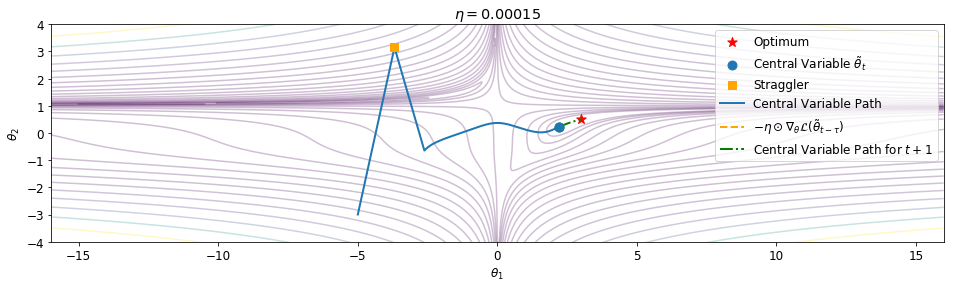
\includegraphics[width=\textwidth]{resources/images/async_straggler_corrected_adag}
  \caption{Correction of the stale worker delta using Equation~\ref{eq:adag}. Contrary to Figure~\ref{fig:async_momentum}, the gradient is scaled down significantly in a way it does not deteriorate the performance of the central variable.}
  \label{fig:adag_straggler_corrected}
\end{figure}

An interesting observation from Chapter~\ref{chapter:accumulated_gradient_normalization}, is that contrary to \textsc{agn}, \textsc{aeasgd} does not show any divergent behaviour for most configurations, i.e., in terms of distributed hyperparameterizations. This is rather interesting, because it tells us that \textsc{aeasgd} has an intrinsic mechanism to deal with parameter staleness. If we review Equation~\ref{eq:aeasgd_worker}, which describes the worker update rule for $\lambda = 1$, we see the that the elastic difference, defined as $\eta_t\rho(\theta^k_t - \tilde{\theta}_t)$, incorperates the \emph{distance} between the worker parameterization $\theta^k_t$ and the \emph{current} parameterization of the central variable $\tilde{\theta}_t$. \textsc{aeasgd} uses the elastic difference as an \emph{opposing force} of the worker exploration, meaning, it limits the amount of exploration that can be done. As a result, the elastic difference of \textsc{aeasgd} in effect limits the \emph{distance} that can be covered by the worker (unless the gradients suddenly become larger). As a result, \textsc{aeasgd} serves as additional evidence for our notion that staleness should be defined in terms of \emph{distance}, and not in terms of stale steps, as formalized in Defination~\ref{def:staleness}.

\begin{definition}{Staleness}
  \label{def:staleness}
  Given a parameterization for worker $k$ at time $t$, $\theta^k_t$, based on the central variable $\tilde{\theta}_{t - \tau}$ where $\tau$ is the number of stale steps, and a central variable at time $t$, $\tilde{\theta}_t$. Then, staleness is defined as the difference (distance) between $\tilde{\theta}_t$ and $\tilde{\theta}_{t-\tau}$.
\end{definition}

Using Definition~\ref{def:staleness}, we can make the deduction that staleness is not really a problem as long as workers commit gradients based on older parameterization of the central variable, which are close to the \emph{current} central variable. This is again additional support for Hypothesis~\ref{hyp:local_optimization}, which states that workers only contribute efficiently to the central variable as they remain close to each other, i.e., the variance of the workers amount the parameter space is small.

\section{Algorithm \& Update Rule}
\label{sec:adag_algorithm}

This Section fully describes the \textsc{adag} update rule, and several architectural decisions that can be made when implementing this technique. Furthermore, using Definition~\ref{def:staleness}, we show how \textsc{adag} can push the limits of asynchronous optimization further, while at the same time eliminating the need for (distributed) hyperparameter gridsearches to ensure convergence.\\

To describe the \textsc{adag} update rule, we use the same terminology and notation used in Definition~\ref{def:staleness} to further strengthen the intuition in parameter staleness, and how parameter staleness is used in Equation~\ref{eq:adag}. Let us consider the case when $\tau = 0$. In this situation, a worker $k$ computes the gradient based on $\tilde{\theta}_{t-\tau}$ which is equal to $\tilde{\theta}_t$. As a result, the distance between these two parameterizations will be 0, which results in the worker delta $\Delta\theta^k$ to be incorperated into the central variable \emph{as is}, and thereby causing the \textsc{adag} update rule to generalize to \textsc{sgd}. In the next step, we add more asynchronous workers to the optimization problem. By doing so, we implicitly increase the staleness as $\mathbf{E}[\tau] = (n - 1)$. As a result, parameter staleness in terms of stale steps, $\tau$, is expected to be larger than 0. Consequently, the distance between $\tilde{\theta}_t$ and $\tilde{\theta}_{t - \tau}$ is \emph{expected} to be non-zero causing the worker delta to be scaled down proportionally to the difference of these parameterizations. However, since parameter changes in Deep Learning usually consist of very small updates, we use the inverse learning rate ($\eta_t^{-1}$) to get a sense of the scale at which these updates operate at. Using the inverse learning rate in Equation~\ref{eq:adag}, and due to the fact that staleness (in terms of distance) is usually relatively small in Deep Learning since the gradients are scaled with respect to $\eta_t$, we find that \textsc{adag} scales the gradients more realistically. Since without the inverse learning rate, the scaling would be very small.

\begin{equation}
  \label{eq:adag}
  \tilde{\theta}_{t+1} = \tilde{\theta}_t + \ddfrac{1}{\eta_t^{-1}\|\tilde{\theta}_t - \tilde{\theta}_{t - \tau}\|^2 + 1} \odot \Delta\theta^k
\end{equation}

Nevertheless, one could view the inverse learning rate from a different perspective. Fist let us denote the set of workers as $\mathcal{W}$. Then, the staleness term in Equation~\ref{eq:adag} can be written as a sequence of gradients from different workers $w$, as shown in Equation~\ref{eq:adag_difference_1}.

\begin{equation}
  \label{eq:adag_difference_1}
  \tilde{\theta}_{t} - \tilde{\theta}_{t - \tau} = \sum_{i = 0}^\tau \exists!\, w \in \mathcal{W}: \eta_t \nabla_\theta \mathcal{L}_w(\tilde{\theta}_{t - \tau_w})
\end{equation}

Furthermore, assuming a static learning rate $\eta$, Equation~\ref{eq:adag_difference_1} can be simplified by moving the learning rate $\eta_t$ before the summation sign, obtaining Equation~\ref{eq:adag_difference_2}.

\begin{equation}
  \label{eq:adag_difference_2}
  \tilde{\theta}_{t} - \tilde{\theta}_{t - \tau} = \eta \sum_{i = 0}^\tau \exists!\, w \in \mathcal{W}: \nabla_\theta \mathcal{L}_w(\tilde{\theta}_{t - \tau_w})
\end{equation}

Remember that the scaling of the worker deltas are proportional to Equation~\ref{eq:adag_difference_3}.

\begin{equation}
  \label{eq:adag_difference_3}
  \eta^{-1} \|\tilde{\theta}_t - \tilde{\theta}_{t - \tau}\|^2
\end{equation}

Substituting the staleness term in Equation~\ref{eq:adag_difference_3} for Equation~\ref{eq:adag_difference_2} gives us:

\begin{equation}
  \label{eq:adag_difference_4}
  \eta^{-1}\|\eta\sum_{i = 0}^\tau \exists!\, w \in \mathcal{W}: \nabla_\theta \mathcal{L}_w(\tilde{\theta}_{t - \tau_w})\|^2
\end{equation}

Earlier, the assumption was made the learning rate is static. As a result, we can cancel the learning rate terms, and thus obtaining Equation~\ref{eq:adag_difference_5}.

\begin{equation}
  \label{eq:adag_difference_5}
  \cancel{\eta^{-1}}\|\cancel{\eta}\sum_{i = 0}^\tau \exists!\, w \in \mathcal{W}: \nabla_\theta \mathcal{L}_w(\tilde{\theta}_{t - \tau_w})\|^2
\end{equation}

This result indicates that the scaling term in Equation~\ref{eq:adag} is proportional to a \emph{unitless} sequence of worker gradients, i.e., not scaled down by a learning rate. As a result, Equation~\ref{eq:adag} is not sensitive to the hyperparameterization of $\eta$. Therefore, the scaling term will work at any scale, and still be proportional to the magnitude of the worker gradients.\\

An additional, but important aspect that needs to be considered is how \textsc{adag} keeps track of $\tilde{\theta}_{t - \tau}$. For this we foresee two possible implementations. The first, described in Algorithm~\ref{algo:adag_1}, keeps track of $\tilde{\theta}_{t - \tau_w}$ for a particular worker $w$ at a worker level. Meaning, worker $w$ keeps track of its local copy $\theta_t^w$, and the original central variable $\tilde{\theta}_{t-\tau}$. Next, when worker $w$ is done computing $\Delta\theta^w_t$, $w$ will commit both $\Delta\theta^w_t$ and $\tilde{\theta}_{t - \tau}$ to the parameter server. Since the parameter server already holds $\tilde{\theta}_{t}$, the parameter server can now compute the next central variable using Equation~\ref{eq:adag}.

\begin{algorithm}[H]
  \caption{Implementation of \textsc{adag} where the workers are responsible for keeping track of $\tilde{\theta}_{t - \tau}$.}
  \label{algo:adag_1}
  \begin{algorithmic}[1]
    \Procedure{ADAGParameterServer}{}
    \State $t \gets 0$ \Comment{Parameter server clock}
    \State $\tilde{\theta}_t \gets \Call{Random}$
    \State
    \Procedure{HandlePull}{$k$} \Comment{$k$ denotes the worker identifier}
    \State \Return $\tilde{\theta}_{t}$
    \EndProcedure
    \State
    \Procedure{HandleCommit}{$k$, $\Delta\theta^w$, $\tilde{\theta}_{t - \tau_k}$}
    \State $\tilde{\theta}_{t + 1} = \tilde{\theta} + \ddfrac{1}{\eta_t^{-1}\|\tilde{\theta}_t - \tilde{\theta}_{t - \tau_k}\|^2 + 1} \odot \Delta\theta^k_t$
    \State $t \gets t + 1$
    \EndProcedure
    \State
    \EndProcedure
  \end{algorithmic}
\end{algorithm}

However, an obvious limitation of Algorithm~\ref{algo:adag_1} is the increased network usage since two parameterizations have to be shipped to the parameter server, i.e., the worker delta $\Delta\theta^k_t$ and the original central variable parameterization $\tilde{\theta}_{t - \tau}$. To reduce the network usage of Algorithm~\ref{algo:adag_1}, and thereby reducing the waiting time of the workers, we propose to let the parameter server keep track of worker pulls, i.e., whenever a worker pulls the central variable, the parameter server copies the central variable into a datastructure (for example, a hashmap), and associates the the parameterization of the central variable with the worker which requested the pull at that time. This procedure is roughly described in Algorithm~\ref{algo:adag_2}. However, we would like to note that despite the fact that Algorithm~\ref{algo:adag_2} reduces the communication costs, it increases the memory requirements proportional to the number of concurrent workers. Which as a result, might be problematic as the number of asynchronous workers is high.

\begin{algorithm}[H]
  \caption{Network efficient implementation of \textsc{adag}.}
  \label{algo:adag_2}
  \begin{algorithmic}[1]
    \Procedure{ADAGParameterServer}{}
    \State $t \gets 0$ \Comment{Parameter server clock}
    \State $\tilde{\theta}_t \gets \Call{Random}$
    \State $m \gets \Call{Initialize}$ \Comment{Initializes a data structure which keeps track of worker pulls.}
    \State
    \Procedure{HandlePull}{$k$} \Comment{$k$ denotes the worker identifier}
    \State $m[k] = \tilde{\theta}_t$
    \State \Return $\tilde{\theta}_{t}$
    \EndProcedure
    \State
    \Procedure{HandleCommit}{$k$, $\Delta\theta^w$}
    \State $\tilde{\theta}_{t + 1} = \tilde{\theta} + \ddfrac{1}{\eta_t^{-1}\|\tilde{\theta}_t - m[k]\|^2 + 1} \odot \Delta\theta^k_t$
    \State $t \gets t + 1$
    \EndProcedure
    \State
    \EndProcedure
  \end{algorithmic}
\end{algorithm}

\section{Experiments}
\label{sec:adag_experiments}

To show the effectiveness of Definition~\ref{def:staleness}, several experiments shall be conducted in the following section regarding the convergence properties of \textsc{adag}. Looking back at Chapter~\ref{chapter:accumulated_gradient_normalization}, we saw that staleness mitigation is critical in highly concurrent environments, as the staleness increases proportionally to the number of workers, as shown in Figure~\ref{fig:staleness_increasing}. Furthermore, without \textsc{adag}, we have to descrease the communication frequency even further to ensure that divergence does not occur. However, as a result of the increased amount of local exploration, parameter updates occur less frequently. Which again results in a slower convergence of the central variable, and thereby reducing the \emph{temporal efficiency} of those highly concurrent configurations compared to less concurrent configurations.

\begin{figure}[H]
  \centering
  \caption{Stalness increasing}
  \label{fig:staleness_increasing}
\end{figure}

\section{Future work}
\label{sec:adag_future_work}
